\section{The robot and its digital twin}
\label{sec:robot}

This chapter turns the inherited mechanical design into a measured plant.
The non-mechanical subsystems are selected first: actuators, battery, compute, sensing and the communication bus.
A digital twin is then derived from the CAD data and validated against the assembled robot.
The parameters the CAD cannot provide, such as the actuator bandwidth, are measured on the real robot to limit the sim2real risk.
The chapter closes with the running speed ceiling the measured plant admits, which \cref{sec:rl} trains against.


\subsection{DASH-01}
\label{sec:machine}

\begin{figure}[htbp]
\centering
\begin{minipage}[c]{0.32\textwidth}
  \centering
  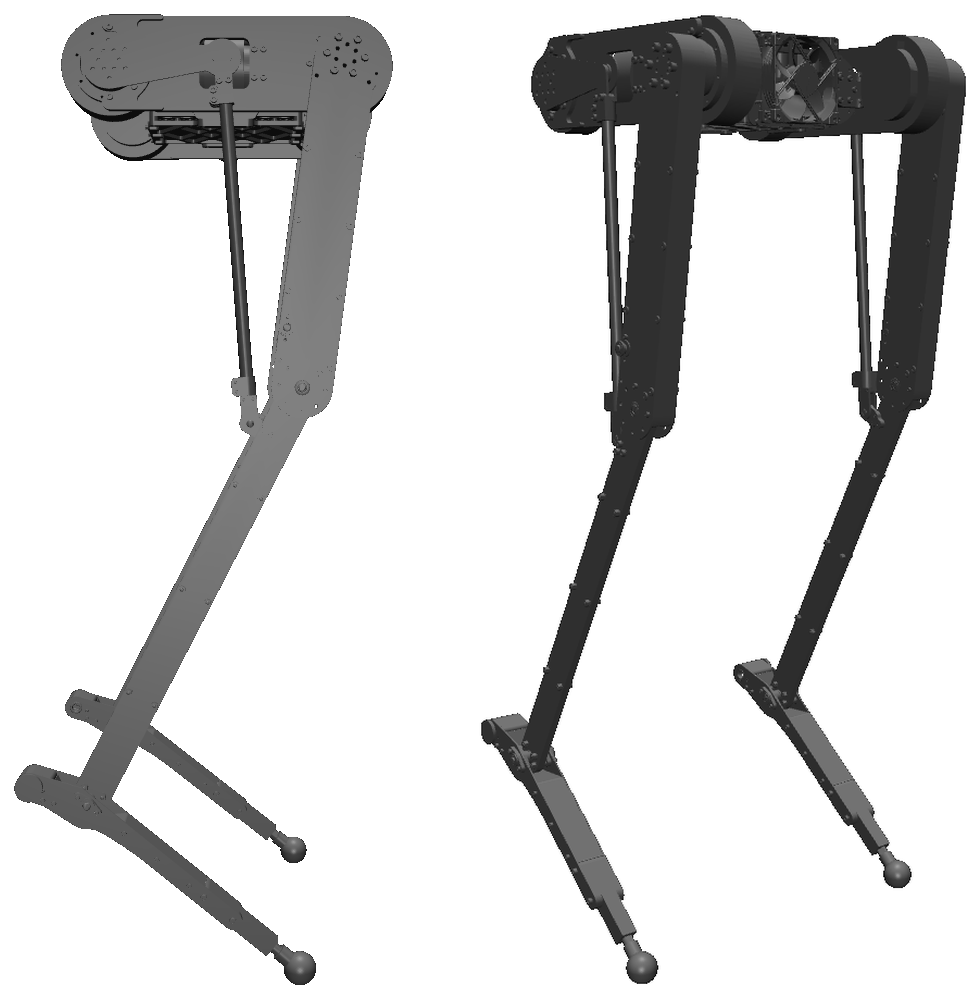
\includegraphics[width=\linewidth]{Figures/fig_robot.png}
\end{minipage}\hfill
\begin{minipage}[c]{0.35\textwidth}
  \centering
  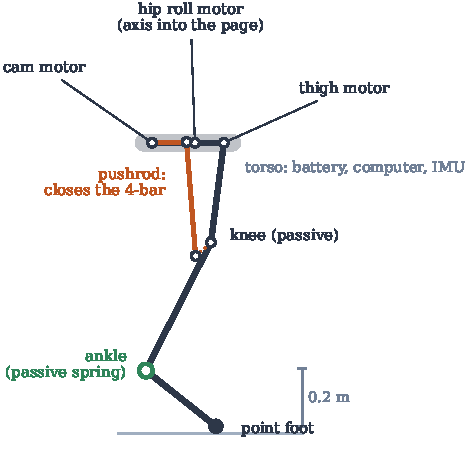
\includegraphics[width=\linewidth]{Figures/fig_leg.pdf}
\end{minipage}
\begin{minipage}[c]{0.22\textwidth}
  \centering
  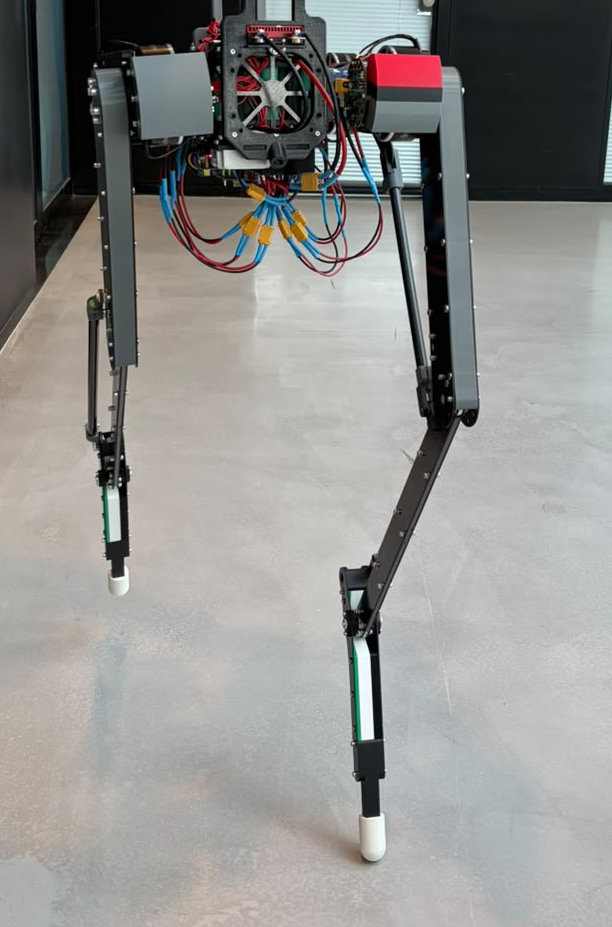
\includegraphics[width=\linewidth]{Figures/dash01-realife.jpg}
\end{minipage}
\caption{DASH-01, Simulated model and real-life picture.}
\label{fig:robot}
\end{figure}

\begin{table}[H]
\centering
\small
\setlength{\tabcolsep}{3.5pt}
\begin{minipage}[t]{0.55\textwidth}
\centering
\begin{tabular}{lcc}
\toprule
& \textbf{Hip roll} & \textbf{Cam, thigh} \\
\midrule
Part & AK60-39 & AKE90-8 \\
Reduction & 39:1 & 8:1 \\
Peak torque, datasheet & 72\,N$\cdot$m & 170\,N$\cdot$m \\
Peak torque, measured & 61.2\,N$\cdot$m & 144.5\,N$\cdot$m \\
Continuous torque & 24\,N$\cdot$m & 55\,N$\cdot$m \\
No-load speed & 10.3\,rad/s & 22.0\,rad/s \\
$K_t$ (N$\cdot$m/A) & 0.12 & 0.272 \\
$R$ ($\Omega$) & 0.60 & 0.164 \\
$K_m$ (N$\cdot$m/$\sqrt{\text{W}}$) & 0.15 & 0.674 \\
Reflected armature (kg$\cdot$m$^2$) & 0.046 & 0.0216 \\
Mass (kg) & 0.75 & 1.40 \\
Unit price (EUR) & 393 & 424 \\
\bottomrule
\end{tabular}
\end{minipage}\hfill
\begin{minipage}[t]{0.43\textwidth}
\centering
\begin{tabular}{lrr}
\toprule
\textbf{Segment} & \textbf{Mass} & \textbf{Count} \\
\midrule
Base & 5764\,g & 1 \\
Hip, with two motors & 3271\,g & 2 \\
Cam & 66\,g & 2 \\
Thigh & 483\,g & 2 \\
Push rod & 71\,g & 2 \\
Ankle spring assembly & 249\,g & 2 \\
Shin & 324\,g & 2 \\
Foot & 222\,g & 2 \\
\midrule
\textbf{Total} & \textbf{15\,136\,g} & \\
\bottomrule
\end{tabular}
\end{minipage}
\caption{The six CubeMars quasi-direct-drive actuators (left) and the weighed segment masses
(right). Measured peak torque is the datasheet figure scaled by the effective joint $K_t$ of
\cref{sec:inertia-validation}. $K_t$ and $R$ are line-to-line, and the motor figure of merit is
$K_m = K_t/\sqrt{R}$. }
\label{tab:motors}
\end{table}

Each leg carries three motors. Hip roll sits at the base, and a cam and a thigh axis drive the
sagittal plane. The knee is passive and follows through the 4-bar. The ankle is passive and follows
through a spring (not rendered). The spring was later measured to be roughly an order of magnitude too soft: at half body weight it deflects 26.6\,deg, which would drive the heel 11.9\,mm through the floor. The ankle was therefore locked in a neutral position with a carbon tube, and the simulation masses were updated to reflect the change.


\newpage 

\subsection{Selecting hardware}
\label{sec:hw-selection}

\subsubsection{Actuators choice}
\label{sec:hw-motor}

A database to select the actuator was assembled.
Major robotic actuator manufacturers' websites were scraped for datasheets and a large language model was used to parse each datasheet.
The database content was then manually checked to ensure the LLM produce the expected result.
The resulting database holds 140 entries across 11 suppliers, listed in \cref{tab:manufacturers}.

\begin{table}[htbp]
\centering
\begin{tabular}{lr}
\toprule
Manufacturer & Actuator count \\
\midrule
ZeroErr       & 32 \\
MyActuator    & 29 \\
CubeMars      & 22 \\
SteadyWin     & 21 \\
Maxon         & 12 \\
MAB Robotics  & 8  \\
RobStride     & 7  \\
HEBI Robotics & 6  \\
Soceboz       & 1  \\
RSL-ETH       & 1  \\
mjbots        & 1  \\
\midrule
Total         & 140 \\
\bottomrule
\end{tabular}
\caption{Actuator manufacturers represented in the database}
\label{tab:manufacturers}
\end{table}

\begin{figure}[H]
\centering
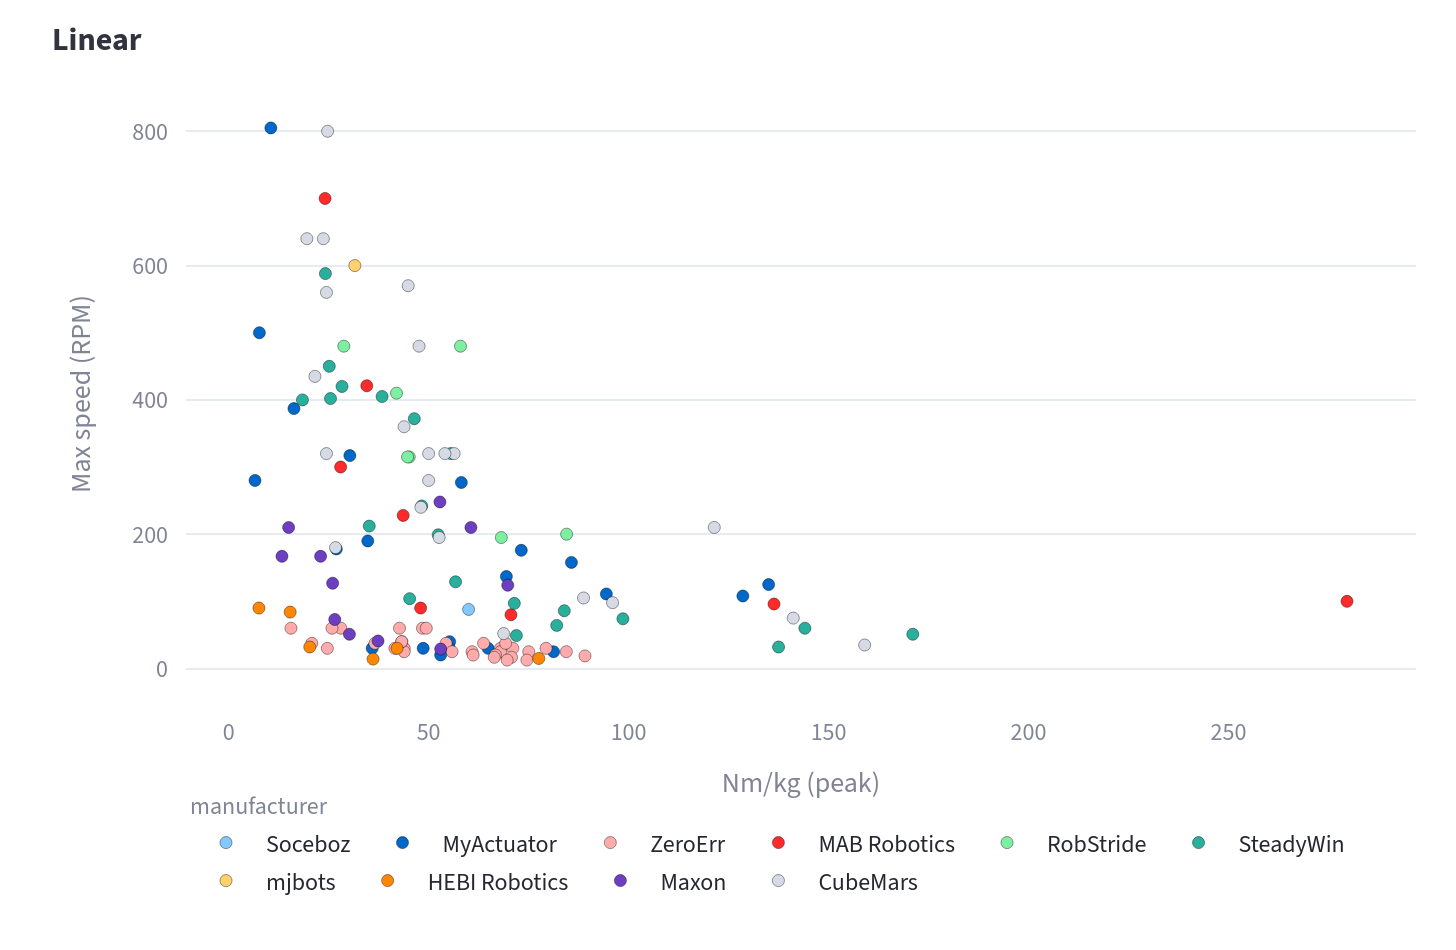
\includegraphics[width=1.05\textwidth]{Figures/ScreenshotActuatorMap.png}
\caption{Excerpt of the dashboard, showing the actuator database used to select the drive.}
\label{fig:motormap}
\end{figure}

The database was compiled into an interactive dashboard, \emph{motormap} \cite{morand2026motormap}, built from the \texttt{actuatorReview} code \cite{morand2026actuatorreview}.
The choice of the actuator itself is detailed in the master's thesis of M. Aebi \cite{aebi2025dash01}.
The final drive choice was the CubeMars AK60-39 for the hip roll and the AKE90-8 for the cam and thigh.
The AKE90-8 is rated for up to 72\,A peak, while the AK60-39 is rated for 17\,A peak.


\subsubsection{Compute, CAN bus and sensing}
\label{sec:hw-compute}

The following \Cref{tab:architecture} summarises the choice of the compute, sensing and network bus.
\begin{table}[H]
\centering
\small
\begin{tabular}{lp{9.3cm}}
\toprule
\multicolumn{2}{l}{\textbf{Compute}} \\
\midrule
Board & Raspberry Pi 3B, stock non-real-time Linux \\
Control loop & 200\,Hz \\
\addlinespace
\multicolumn{2}{l}{\textbf{Sensing}} \\
\midrule
IMU & ICM-20948, 10-axis, on a Waveshare Sense HAT\,(B) \\
IMU interface & I2C, $\pm4$\,g, $\pm1000$\,dps, 200\,Hz sampling \\
Analog input & 4-channel ADC on the same HAT \\
\addlinespace
\multicolumn{2}{l}{\textbf{Network bus}} \\
\midrule
Controller & \texttt{mcp251xfd} over SPI, dual-channel CAN HAT \\
Topology & two independent 1\,Mbit buses, one per leg \\
Measured load & 26\,\% of each of the two buses (polled at 200\,Hz) \\
\bottomrule
\end{tabular}
\caption{The robot's non-mechanical architecture: compute, sensing and the CAN network
bus.}
\label{tab:architecture}
\end{table}


\label{sec:compute-choice} The board is a \textbf{Raspberry Pi 3
Model B}, running stock non-real-time Linux. It was chosen over the laboratory's usual BeagleBone
Black for its faster SSH sessions and its four cores, which let the control loop and the data
processing run side by side.
An \texttt{mcp251xfd} controller over SPI provides CAN as two independent 1\,Mbit buses, one per leg.
The Pi also hosts a WiFi access point and the web interface of \cref{sec:deploy}, through which most measurements in \cref{sec:plant-id} were taken.

\Cref{sec:plant-id-timing} presents the measured timing of the control loop and the CAN bus.

Aside from the motor encoders and current feedback, the only proprioceptive sensor is the IMU located on the base of the robot.
Contact sensors were considered and never fitted due to lack of time.
The IMU unit is an \textbf{ICM-20948} on a Waveshare Sense HAT\,(B), read over I2C. 


\subsubsection{Battery choice}
\label{sec:hw-battery}

A database of roughly 430 commercial cells was built on the same principle as the actuator database.
Since 48\,V is the highest pack voltage the selected drives accept, the database was filtered to cells usable in a 13S configuration.
The motor selection sets the current requirement. Assuming half of the six motors at peak torque simultaneously (two AKE90-8 and one AK60-39), the pack must deliver about 160\,A.
From these candidates, a 13S2P pack of EVE INR21700-50PL cells was selected, as the best compromise between energy density, power density and cost.

The pack can be monitored over Bluetooth and its limits configured there with the DALY BMS app.
A CAN interface is also available but was not used, due to lack of time.

The manufacturer states the internal resistance below 10\,m$\Omega$ per cell, which gives about 65\,m$\Omega$ for the 13S2P pack.
At the rated 360\,A peak, the voltage drop would reach 23\,V.
At the 160\,A working peak of the motor budget, the drop is about 10\,V, which the BMS low-voltage protection tolerates on a full charge.
Due to the lack of voltage feedback on the drives, this figure has not been verified on the real robot.
\begin{table}[htbp]
\centering
\small
\setlength{\tabcolsep}{4pt}
    \begin{tabular}{lp{3.5cm}}
        \toprule
        \textbf{Parameter} & \textbf{Specification} \\
        \midrule
        Cell & EVE INR21700-50PL, 5.0\,Ah \\
        Configuration & 13S2P \\
        Nominal voltage, capacity & 48.1\,V, 10\,Ah (468\,Wh) \\
        Continuous rating & 100\,A, cell-limited \\
        Peak current & 360\,A for 2\,s\\
        Mass (BMS, casing) & 3.5\,kg \\
        Power density (peak) & 4900\,W/kg \\
        Power density (cont.) & 1370\,W/kg \\
        Energy density & 133.7\,Wh/kg \\
        \bottomrule
    \end{tabular}
\caption{Specification of the selected 13S2P battery pack.}
\label{tab:battery-spec}
\end{table}

\begin{figure}[H]
\centering
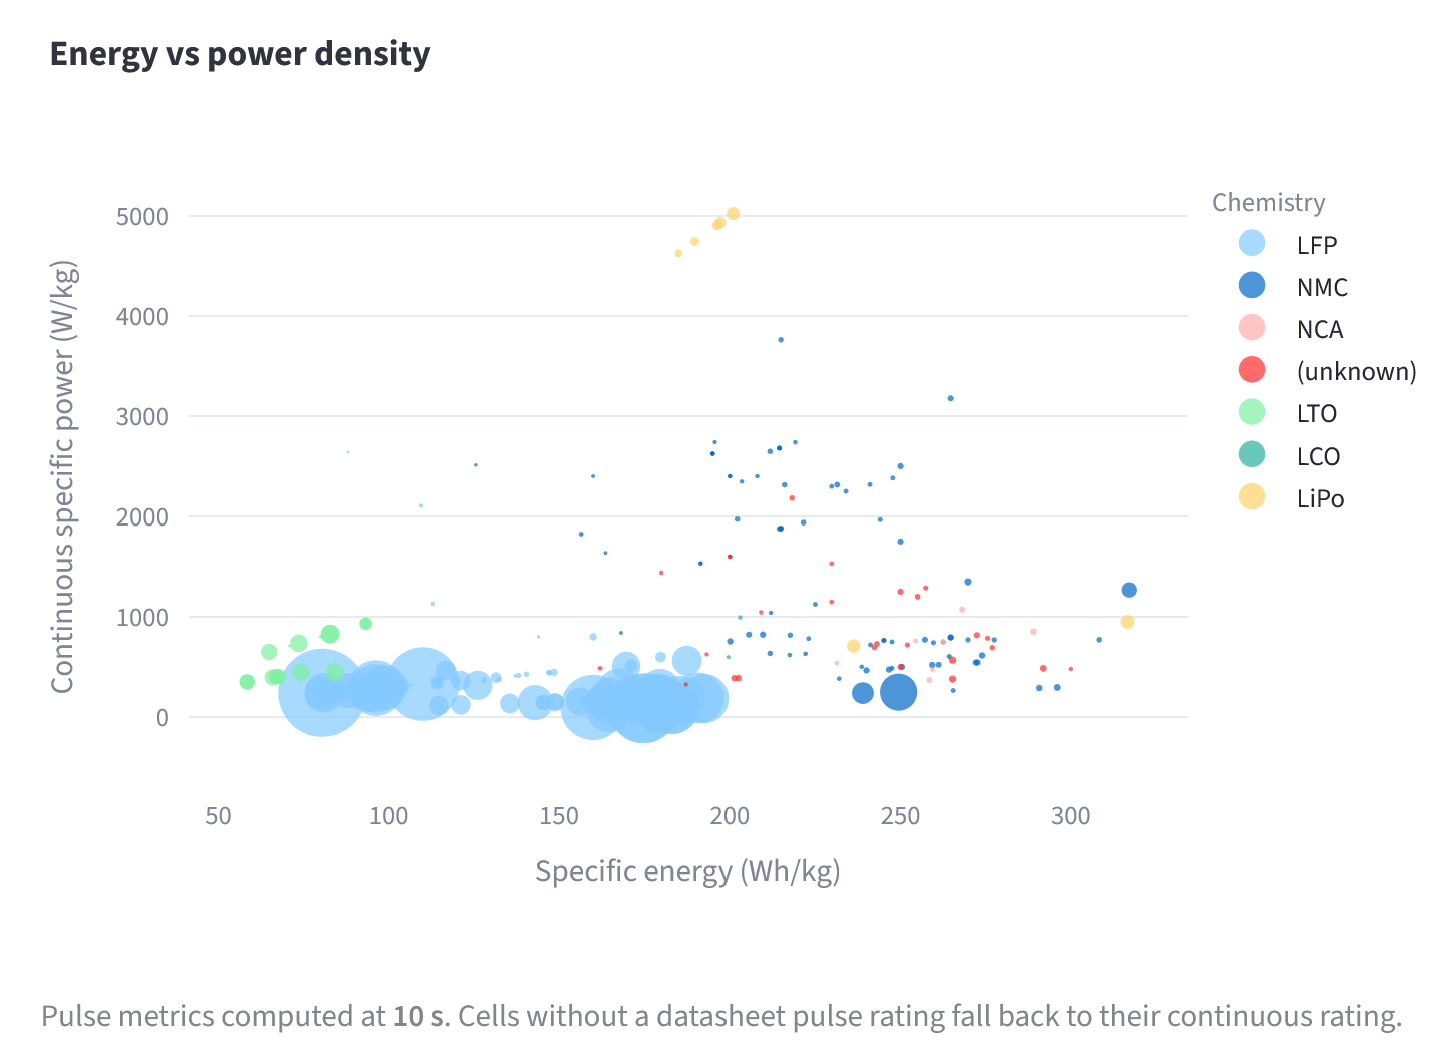
\includegraphics[width=1\textwidth]{Figures/cellDashboard.png}
\caption{Excerpt of the dashboard, showing the cell database used to select the pack.}
\label{fig:celldashboard}
\end{figure}

\newpage


\subsection{The digital twin}
\label{sec:twin}
A simulation ready model was derived from the CAD data. The model is exported in two formats, URDF and MJCF.
The detailed procedure to export the model is described in the appendix (\cref{sec:app-pipeline}).
This took a lot of time and effort due to lack of experience and the poor documentation of the plugin used to export the model.
The final recipe consisted of exporting each segment of the robot as a STEP file with the origin at the joint (except for the base which was in its centre).
Care was taken to ensure the reference axes were aligned in a consistent manner across the segments.
The robot model was reassembled in Autodesk Fusion 360 and exported to URDF using the ACDC4Robot plugin~\cite{qiu2024describing}.
The kinematic loop was broken in the URDF and closed in the MJCF using an equality constraint between two sites, one on the pushrod and one on the shin.
This was necessary because URDF is a tree format and cannot express kinematic loops.

\subsection{Digital twin validation and plant identification}
\label{sec:plant-id}
The digital twin is validated against the real robot for the kinematic and dynamic properties.
The model is also refined with measured parameters that cannot be accurately estimated from the CAD model, to reduce the sim2real gap.

\subsubsection{Joint Limits validation}
\label{sec:sim-hygiene}

The cam and thigh joints close a passive 4-bar loop through the pushrod and knee. Their safe ranges
do not compose into two independent intervals: a per-joint minimum and maximum would allow poses
the mechanism cannot assemble. The safe envelope is instead derived directly in actuator space.
Each leg's three drives are held current-free and the leg is backdriven by hand through its full
travel, logging the raw actuator angles \cite{morand2026runningrobot}.

\Cref{fig:joint-limits-actuator} shows the result for both legs: a plain interval for hip roll, and
a two-dimensional band for the coupled (cam, thigh) pair. The demonstrated hip roll range spans
42.8\,deg to 126.1\,deg on the left leg and 66.5\,deg to 147.7\,deg on the right; both are eroded by
3\,deg for a safety margin and the eroded interval is stored as the hip roll limit. For the knee pair,
the recorded (cam, thigh) samples are rasterised onto a 1\,deg grid, dilated to close small sampling
gaps, then eroded by the same 3\,deg margin. The stored safe region covers 11.0\,\% of its own
bounding box on the left leg and 9.4\,\% on the right, confirming the band is far from rectangular.
The onboard safety layer checks every commanded pose against this grid before it reaches the drives
(\cref{sec:safety}).

\begin{figure}[H]
\centering
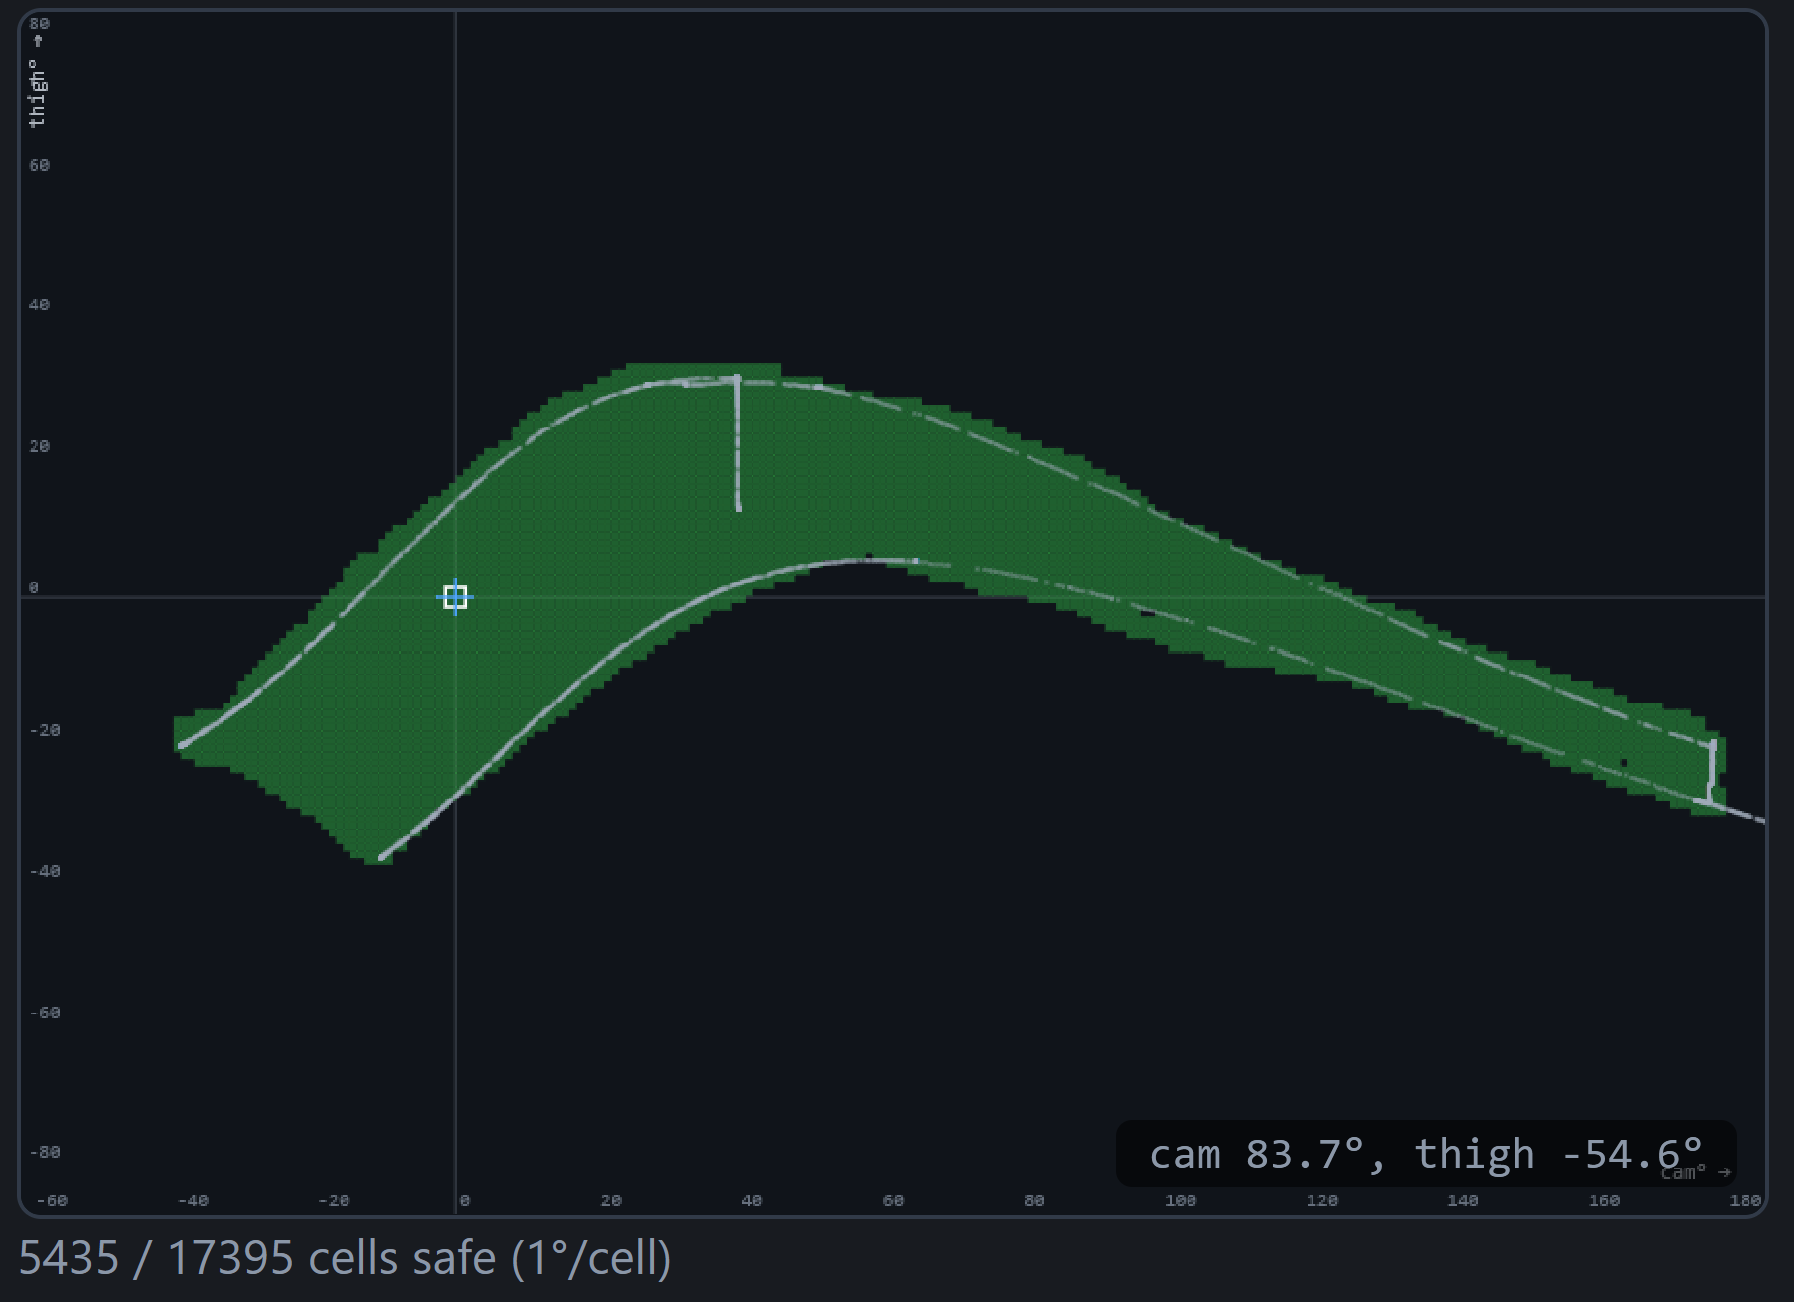
\includegraphics[width=0.95\linewidth]{Figures/fig_workspace_joint.png}
\caption{Joint-limit validation in actuator space: the coupled (cam, thigh) 4-bar band, backdriven by hand for each leg.
The green region is the safe envelope enforced by the onboard safety layer.}
\label{fig:joint-limits-actuator}
\end{figure}
\subsubsection{Inertia matrix validation}
\label{sec:inertia-validation}

The CAD export provides, for every body $b$, a mass $m_b$, a centre of mass $\mathbf r_{c,b}$ and an
inertia tensor $\mathbf I_b$, all expressed in the body frame. A wrong export transformation rotates
$\mathbf r_{c,b}$ and $\mathbf I_b$ without changing their magnitude, so the check below has to be
sensitive to the frame and to the magnitude separately.

Each actuated joint's torque constant $K_t$, effective inertia $I_{\mathrm{eff}}$ and friction
(viscous $b_v$, Coulomb $b_c$) are identified from two excitation profiles logged through the web
interface \cite{morand2026runningrobot}: a quasi-static sine sweep at 0.03\,Hz, which holds the
joint near equilibrium so gravity dominates the measured torque, and a 20\,s chirp from 0.05 to
0.6\,Hz, which excites the inertial term. Every joint obeys the single-DOF balance
\begin{equation}
K_t\,(i - i_0) = I_{\mathrm{eff}}\,\ddot q + b_v\,\dot q + b_c\,\mathrm{sgn}(\dot q) + \tau_g(\mathbf q),
\label{eq:joint-balance}
\end{equation}
where $i$ is the phase current, $i_0$ the drive's DC current offset and $\tau_g(\mathbf q)$ the
model's gravity torque at that joint, a function of the full configuration $\mathbf q$.

The gravity torque is computed from the inertial data by forward kinematics only, which stays
well-posed at the 4-bar singularity where inverse dynamics does not (\cref{sec:twin}). With
$\mathbf J_{c,b}(\mathbf q)$ the centre-of-mass Jacobian of body $b$ and $\mathbf g$ the gravity
vector, the gravity generalised force on all joints, actuated ($a$) and passive ($p$), is
\begin{equation}
\boldsymbol\tau_g(\mathbf q) = -\sum_b m_b\,\mathbf J_{c,b}^{\!\top}(\mathbf q)\,\mathbf g .
\label{eq:grav-torque}
\end{equation}
The closed loop couples the two sets. Linearising the loop-closure constraint,
$\mathbf J_a\,\delta\mathbf q_a + \mathbf J_p\,\delta\mathbf q_p = \mathbf 0$, gives the
passive-to-actuated map
\begin{equation}
\mathbf G = \frac{\partial \mathbf q_p}{\partial \mathbf q_a}
          = -\bigl(\mathbf J_p^{\!\top}\mathbf J_p + \lambda\mathbf 1\bigr)^{-1}\mathbf J_p^{\!\top}\mathbf J_a,
\qquad \lambda = 10^{-6},
\label{eq:loop-jacobian}
\end{equation}
damped so that it stays bounded at the singular poses, and by virtual work the gravity torque seen
by the actuated joints is the reduced-coordinate projection
\begin{equation}
\boldsymbol\tau_{g,a}^{\mathrm{red}} = \boldsymbol\tau_{g,a} + \mathbf G^{\!\top}\boldsymbol\tau_{g,p}.
\label{eq:grav-reduced}
\end{equation}
This is the $\tau_g$ used in \cref{eq:joint-balance} for the cam and thigh joints, which drive the
leg through the 4-bar; abduction is loop-independent.

Dividing \cref{eq:joint-balance} by $K_t$ makes it linear in the measured quantities. For the $N$
pooled samples of one joint, the regressor matrix $\boldsymbol\Phi \in \mathbb R^{N\times 5}$ and the
parameter vector $\boldsymbol\theta$ are
\begin{equation}
\boldsymbol\Phi_{k,:} = \begin{bmatrix} \ddot q_k & \dot q_k & \mathrm{sgn}(\dot q_k) & \tau_g(\mathbf q_k) & 1 \end{bmatrix},
\qquad
\boldsymbol\theta = \begin{bmatrix} I_{\mathrm{eff}}/K_t & b_v/K_t & b_c/K_t & 1/K_t & i_0 \end{bmatrix}^{\!\top},
\label{eq:regressor}
\end{equation}
and the estimate is the ordinary least-squares solution
\begin{equation}
\hat{\boldsymbol\theta} = \arg\min_{\boldsymbol\theta}\;\bigl\|\boldsymbol\Phi\,\boldsymbol\theta - \mathbf i\bigr\|_2^2
                        = \boldsymbol\Phi^{+}\,\mathbf i,
\label{eq:ls-fit}
\end{equation}
with $\mathbf i$ the stacked current samples. The quasi-static and chirp runs are simply
concatenated. The $\tau_g$ column varies with pose across the slow sweep and fixes
$K_t = 1/\hat\theta_4$; the $\ddot q$ column is large only during the chirp and fixes
$I_{\mathrm{eff}} = \hat\theta_1 K_t$; the friction terms follow from $\hat\theta_2$ and
$\hat\theta_3$. The intercept column is essential: over a short sweep $\tau_g$ is itself mostly
constant, so without it the drive's current offset lands in $\hat\theta_4$ and can flip the sign of
$K_t$. The inertia tensors enter through the second column: the tree mass matrix $\mathbf M(\mathbf q)$
built from the $\mathbf I_b$ gives the link contribution, and the rotor armature is the remainder
$J_{\mathrm{rot}} = I_{\mathrm{eff}} - M_{jj}(\bar{\mathbf q})$ at the median pose $\bar{\mathbf q}$.

A raw torque residual is hard to judge on its own, so it is converted into a mass-equivalent error,
\begin{equation}
\epsilon_m = \frac{\mathrm{RMS}\bigl(K_t(i_k - i_0) - \hat\tau_k\bigr)}{\mathrm{RMS}\bigl(\tau_g(\mathbf q_k)\bigr)},
\qquad
\hat\tau_k = I_{\mathrm{eff}}\,\ddot q_k + b_v\,\dot q_k + b_c\,\mathrm{sgn}(\dot q_k) + \tau_g(\mathbf q_k),
\label{eq:mass-error}
\end{equation}
the fraction of the gravity torque the model fails to explain, read as a relative error on the
segment masses. It is an upper bound, since a part of the residual is friction rather than gravity
torque. \Cref{fig:inertia-validation} reports the per-joint values. The relative error is large
because the segment masses are small, so their gravity torque sits close to the noise floor.

The check still serves its purpose. $K_t$ and the gravity model enter \cref{eq:joint-balance} only
through their product, so the fit alone cannot tell a scaled $K_t$ from a scaled mass; frame and
magnitude are therefore tested separately. The pose dependence of $\tau_g$ tests the frame of
$\mathbf r_{c,b}$, since a mis-rotated centre of mass changes the shape of the gravity curve and not
only its size. The recovered $K_t$ against the datasheet value tests the magnitude. Both confirm
that the inertial data are in the correct frame and of the correct magnitude, and that the gravity
trend is right. Since the CAD values are not random, a correct frame and magnitude imply the export
transformation is correct, and the CAD inertia data can be trusted. The bounded mass error
$\epsilon_m$ is reused as a domain-randomisation range in the RL training, to make the policy
robust to this uncertainty.

\begin{figure}[H]
\centering
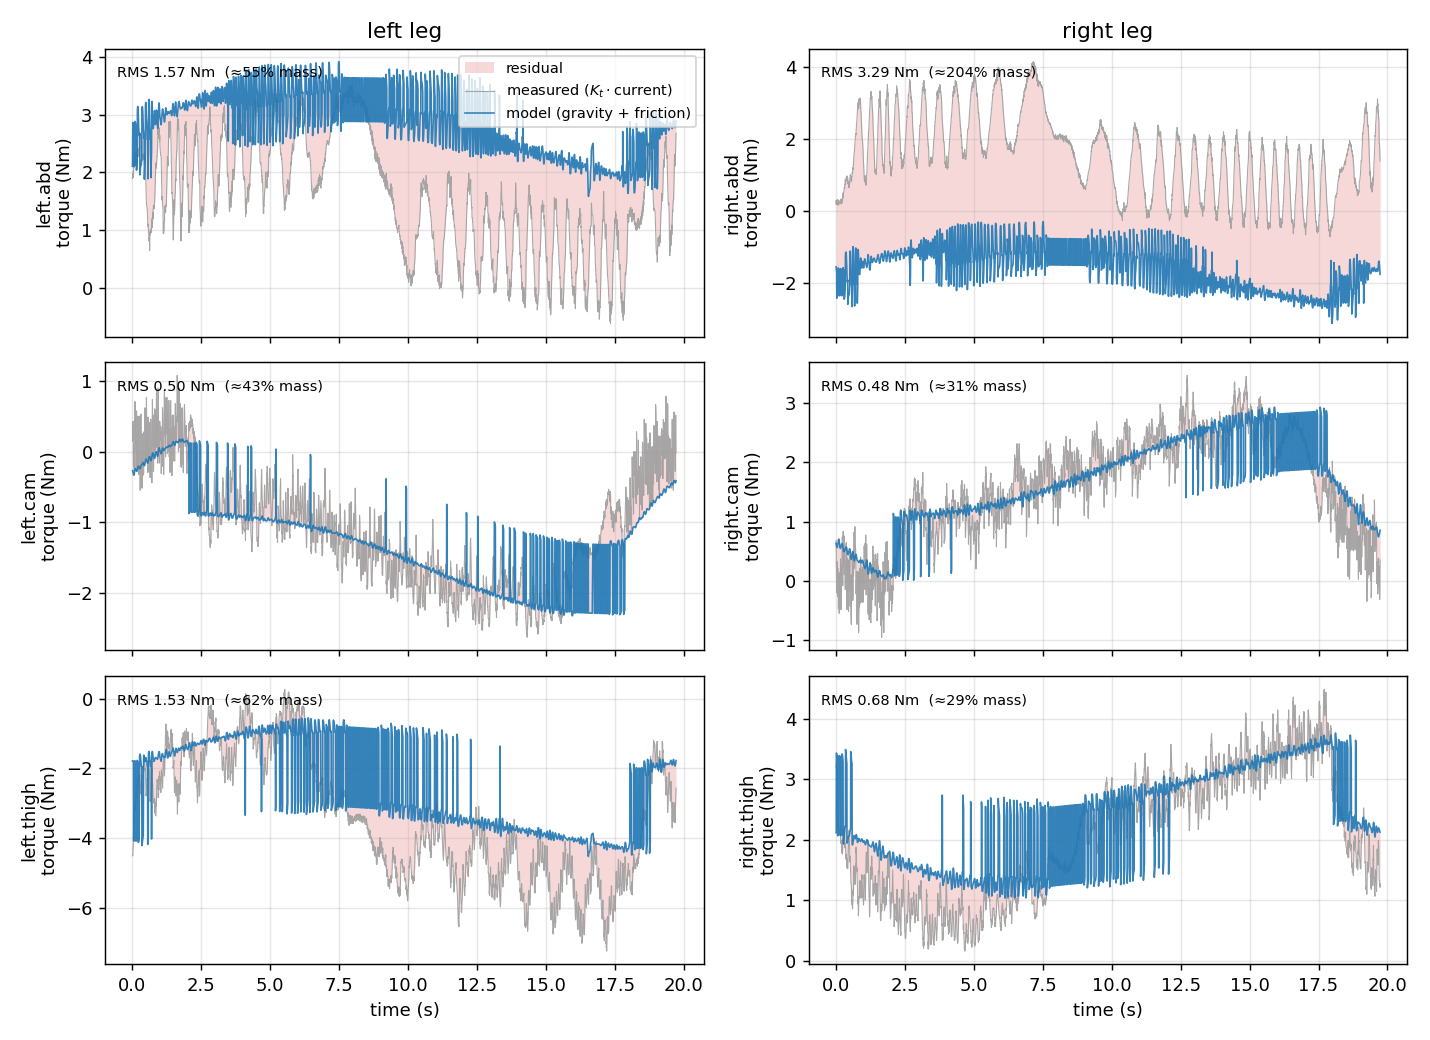
\includegraphics[width=0.9\linewidth]{Figures/inertiaValidationGravity.png}
\caption{Gravity-model validation on the slow (0.03\,Hz) quasi-static sweep: measured torque
($K_t$ times current) against the model's predicted torque (gravity plus friction), residual shaded,
per joint. The mass-equivalent error is the RMS residual divided by the RMS gravity torque. The fast
ripple is likely the P-only position loop's stick-slip response due to friction.}
\label{fig:inertia-validation}
\end{figure}


\subsubsection{CAN bus latency and load characterisation}
\label{sec:plant-id-timing}
The whole control loop was benchmarked on the robot with the web interface running.
These results were reused in the RL curriculum to make the policy robust to the timing jitter.

\begin{table}[htbp]
\centering
\small
\begin{tabular}{lrrrrr}
\toprule
\textbf{Rate} & \textbf{Mean period} & \textbf{Jitter (sd)} & \textbf{p99} & \textbf{Max} & \textbf{Budget used} \\
\midrule
50\,Hz  & 20.148\,ms & 2.151\,ms & 22.41\,ms & 49.29\,ms & 23\,\% \\
100\,Hz & 10.000\,ms & 0.251\,ms & 10.40\,ms & 12.28\,ms & 37\,\% \\
\textbf{200\,Hz} & \textbf{5.000\,ms} & \textbf{0.141\,ms} & \textbf{5.21\,ms} & 7.46\,ms & \textbf{50\,\%} \\
400\,Hz & 2.504\,ms & 0.193\,ms & 3.24\,ms & 5.13\,ms & 73\,\% \\
\bottomrule
\end{tabular}
\caption{Measured closed-loop timing on the robot's Raspberry Pi 3B, with the web interface competing for CPU.
One tick drains both CAN buses, runs a dummy inference of the policy and writes all the motor commands.}
\label{tab:loop-timing}
\end{table}

At 50\,Hz the mean period overshoots its 20\,ms target and the jitter is an order of magnitude above the faster rates.
The likely cause is the non-real-time scheduler, which wakes the loop late after the longer sleeps.
The dummy inference was later found to be too optimistic: the real policy requires the loop to run at 100\,Hz on the Pi 3B.


\subsubsection{IMU characterisation}
The base IMU was sampled at rest for 300\,s, configured at $\pm4$\,g and $\pm1000$\,dps, with a
50\,Hz internal low-pass and 200\,Hz sampling.
The measurement gives 1.8\,mg and 0.08\,dps RMS noise. The noise density is
218\,$\mu$g/$\sqrt{\text{Hz}}$ and 0.0096\,dps/$\sqrt{\text{Hz}}$. The gyro turn-on bias is
repeatable at $[1.03, 0.11, -0.53]$\,dps, and the in-run bias stability is 0.010--0.012\,dps.

\begin{figure}[H]
\centering
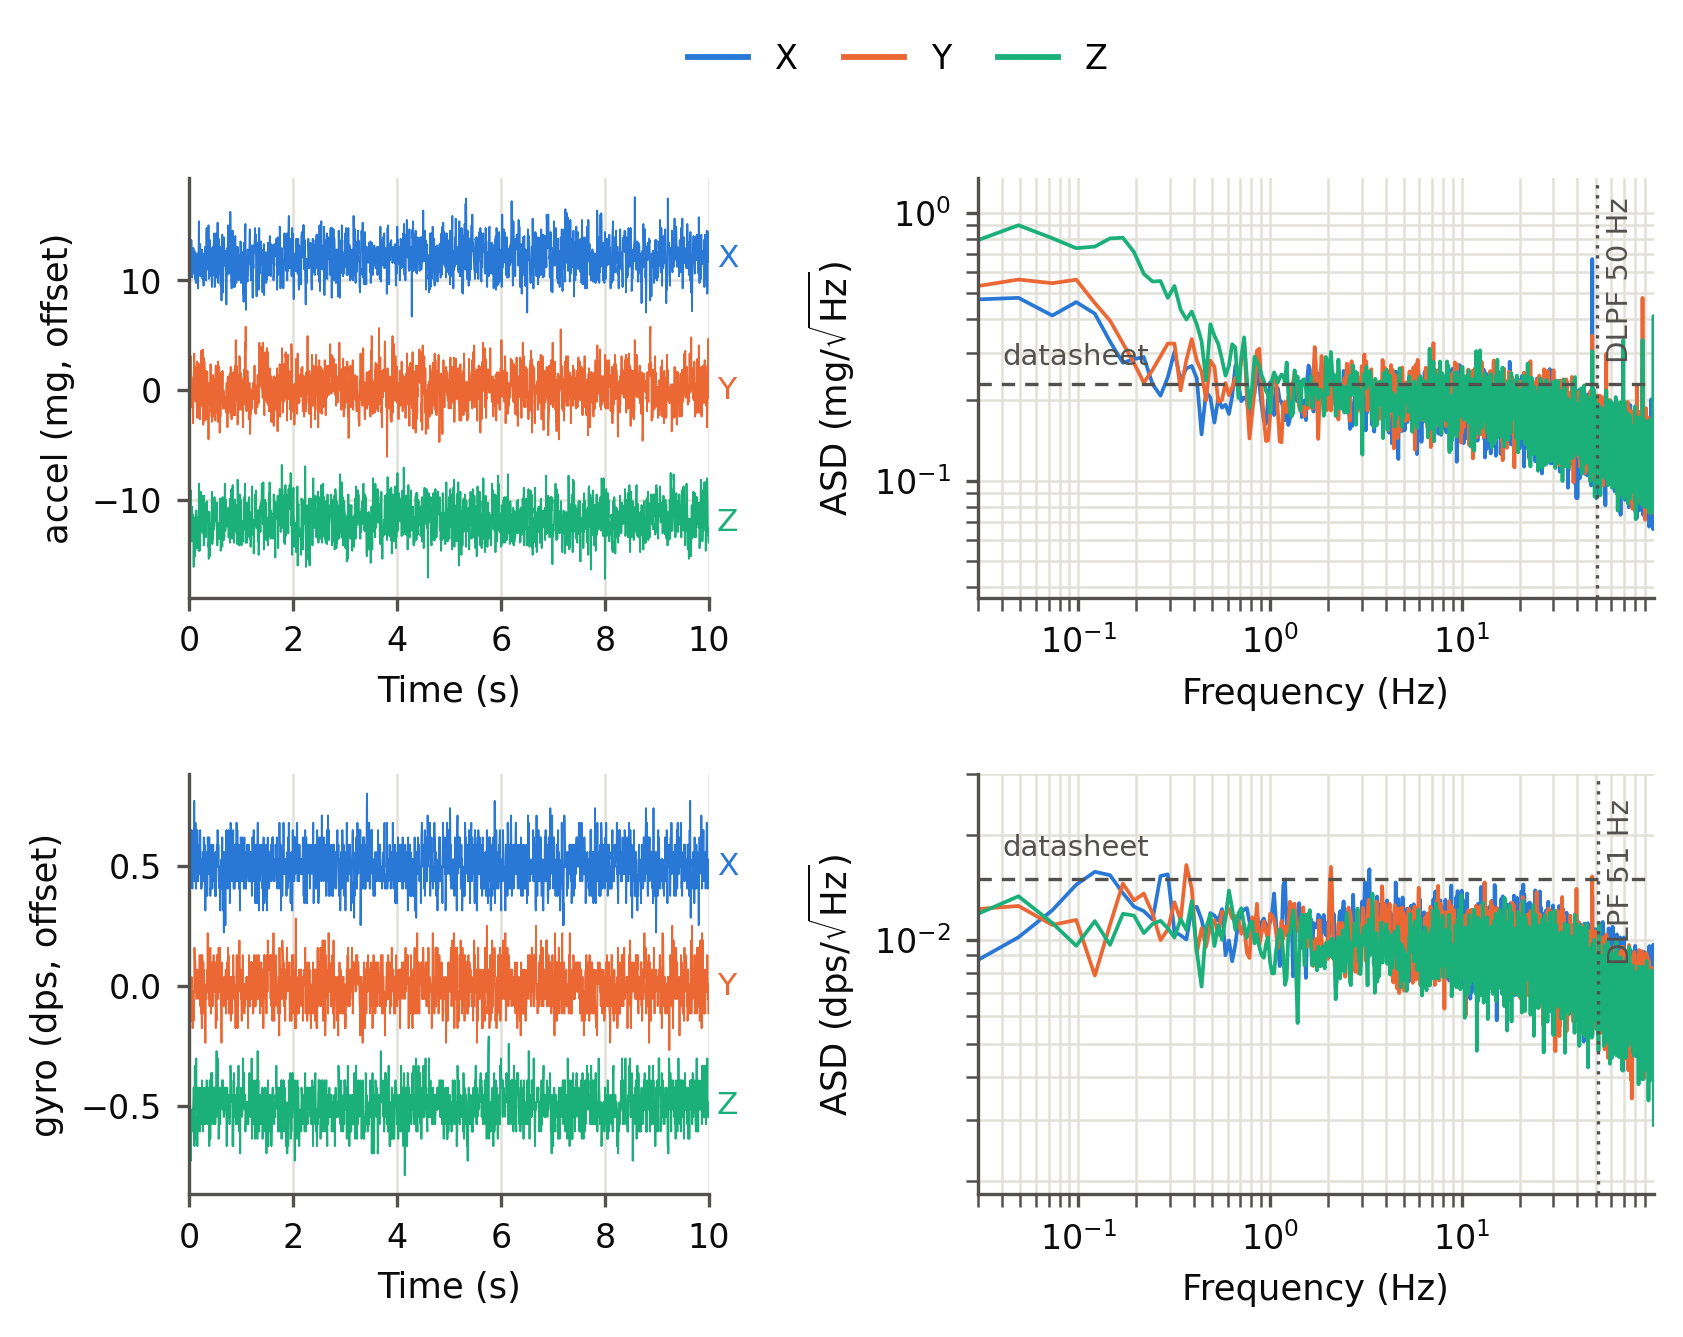
\includegraphics[width=0.9\linewidth]{Figures/fig_imu_noise.png}
\caption{Noise characterisation of the base IMU (ICM-20948), sampled at 200\,Hz for 300\,s at rest.}
\label{fig:imu-noise}
\end{figure}


\subsubsection{Actuator thermal characterisation}

The actuator thermal response was not measured due to lack of time. The thermal lumped model parameters were estimated roughly from the mass of the actuator but not used in the simulation.

\subsubsection{Battery characterisation}

The battery was not characterised due to lack of time; its behaviour was estimated from the datasheet internal resistance of the cell.
This is further complicated by the lack of voltage feedback on the drives, which prevents measuring the voltage drop under load.
In practice, this is not expected to be a problem: the drives are not used in torque control, so they can be expected to regulate the voltage drop without taking the RL policy out of its distribution.

\newpage 

\subsubsection{Actuator bandwidth characterisation}
\label{sec:plant-id-drive}

The AKE90-8's closed-loop position bandwidth was measured in both Servo and MIT mode, on the
thigh joints of both legs, with the legs attached but unloaded (robot homed on its stand). Both are position loops at the interface each mode is actually used through, so the two are
directly comparable. In Servo mode the command is a position set-point to the drive's internal
position loop. In MIT mode the drive runs its impedance law
\begin{equation}
\tau = k_p\,(p_{\mathrm{des}} - p) - k_d\,\dot p,
\qquad k_p = 200\ \mathrm{N\,m/rad},\quad k_d = 5\ \mathrm{N\,m\,s/rad},
\label{eq:mit-impedance}
\end{equation}
with the feed-forward velocity and torque held at zero. These are the deployed gains, the same
$\langle k_p, k_d\rangle$ actuator the policy is trained against in simulation
(\cref{sec:twin}). One extra run at $k_p = 500$ probes the stiffness dependence.

The excitation is a stepped sine, so that every frequency is measured in
steady state: 1 to 30\,Hz in 1\,Hz steps, at least 5\,s inside each frequency, with the frequency
switched at upward zero crossings so the command stays continuous. The command amplitude follows
\begin{equation}
A(f) = \min\!\Bigl(A_{\max},\ \frac{v_{\max}}{2\pi f}\Bigr),
\qquad A_{\max} = 0.044\ \mathrm{rad},\quad v_{\max} = 1\ \mathrm{rad/s},
\label{eq:bode-amplitude}
\end{equation}
constant position amplitude at low frequency and constant velocity amplitude above the corner, so
that neither excursion nor speed grows with frequency. Commands are streamed at 200\,Hz over CAN
and the drive's reported position, at the same rate and kernel time-stamped on reception, is the
measured output; its resolution is 0.1$^\circ$. A 200\,Hz watchdog aborts on drive error,
over-current, over-temperature or position leaving the safe window \cite{morand2026runningrobot}.

Per frequency, the first 1.2\,s after each switch are discarded and the reported position $p_k$
is projected by least squares onto the command's own sine and cosine, plus a mean and a linear
drift term,
\begin{equation}
p_k \approx a\,\sin\varphi_k + b\,\cos\varphi_k + c + d\,t_k,
\qquad
|H(f)| = \frac{\sqrt{a^2 + b^2}}{A(f)},\quad
\angle H(f) = \operatorname{atan2}(b, a),
\label{eq:bode-fit}
\end{equation}
where $\varphi_k$ is the command phase at sample $k$. Fitting on the exact command phase, instead of
an FFT bin, rejects the drift and the quantisation noise. Points whose response amplitude
falls below the position-feedback resolution, or whose residual exceeds 45\,\% of the response,
are masked since they are likely noise; the high-frequency Servo points end there by design. The
$-3$\,dB frequency is read by linear interpolation of the magnitude, and the loop delay from the
slope of the unwrapped phase above 4\,Hz,
$\tau_d = -\tfrac{1}{360^\circ}\,\mathrm{d}\angle H/\mathrm{d}f$.

\Cref{fig:actuator-bode} shows the results. Servo mode reaches $-3$\,dB at 1.9\,Hz on both thighs.
MIT mode reaches $-3$\,dB at 6.1 to 6.5\,Hz at the deployed gains, and 18\,Hz at $k_p = 500$ with
the same $k_d$: the corner scales with $k_p/k_d$, so the loop is damping-dominated. The phase
slope gives a delay of 11 to 13\,ms in MIT mode against 19 to 22\,ms in Servo mode.

\begin{figure}[H]
\centering
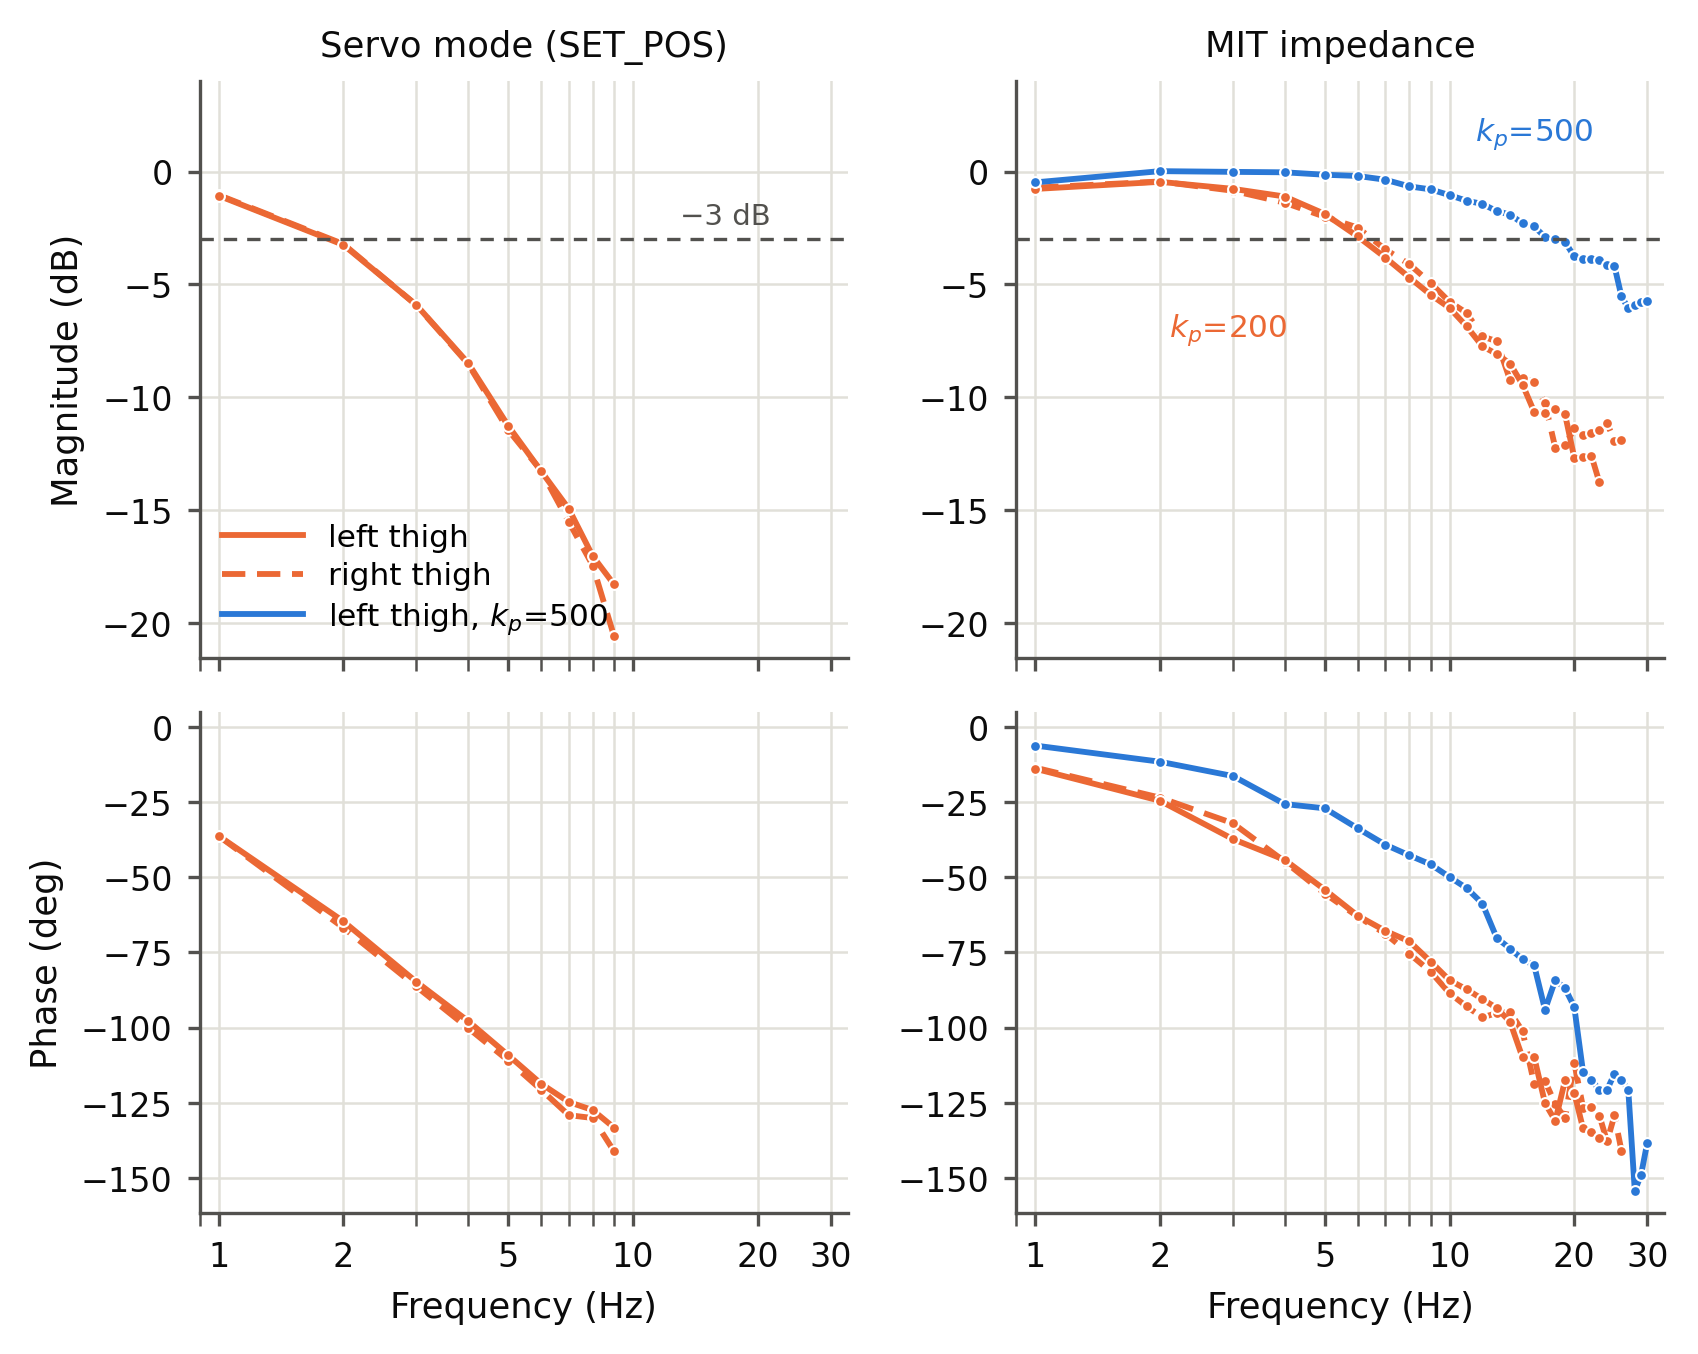
\includegraphics[width=0.75\linewidth]{Figures/actuator_bode.png}
\caption{Measured closed-loop position frequency response of the AKE90-8 thigh drives, both
legs, stepped-sine excitation 1--30\,Hz with legs attached and unloaded: Servo mode's internal
position loop against MIT mode's impedance loop at the deployed gains ($k_p = 200$, $k_d = 5$),
plus one MIT run at $k_p = 500$. Points below the 0.1$^\circ$ feedback resolution are masked.}
\label{fig:actuator-bode}
\end{figure}

\subsection{Deployment stack}
\label{sec:deploy}

The policies of \cref{sec:rl} have to run somewhere. To streamline the process and simplify the measurement of the plant parameters, a web interface was built on the robot.
A systemd entry starts the web interface at boot. The Raspberry Pi acts as a WiFi access point (SSID \texttt{runningmachine}, password \texttt{runningmachine}).
Once connected to the network, the web interface is reachable at \texttt{http://192.168.4.1:8080/}.

\subsubsection{Calibration sequence}
\label{sec:calibration}
The actuators do not hold their position when powered off, so a calibration sequence is needed to zero the joints.
The user needs to hold the robot in a known configuration and run the calibration sequence which registers the current joint position as zero.
The user then needs to move each joint in a specific direction and check that the angle increases (otherwise, the joint direction needs to be inverted by clicking a button in the web interface).
Once the robot is zeroed, the workspace can be registered by backdriving the robot and recording the joint position at the limit of the workspace.
The web UI then cleans the measurement to show the boundary and the user can draw / fill the safe workspace in the web interface.
This is used to limit the joint position in the safety layer.

The IMU is also calibrated in the web interface by holding the robot still and recording the bias of the accelerometer and gyroscope.
To ensure the axes are aligned, the user needs to move the robot around a given axis of the base and check that the correct axis is increasing.

\begin{figure}[H]
\centering
\begin{minipage}[t]{0.48\linewidth}
\centering
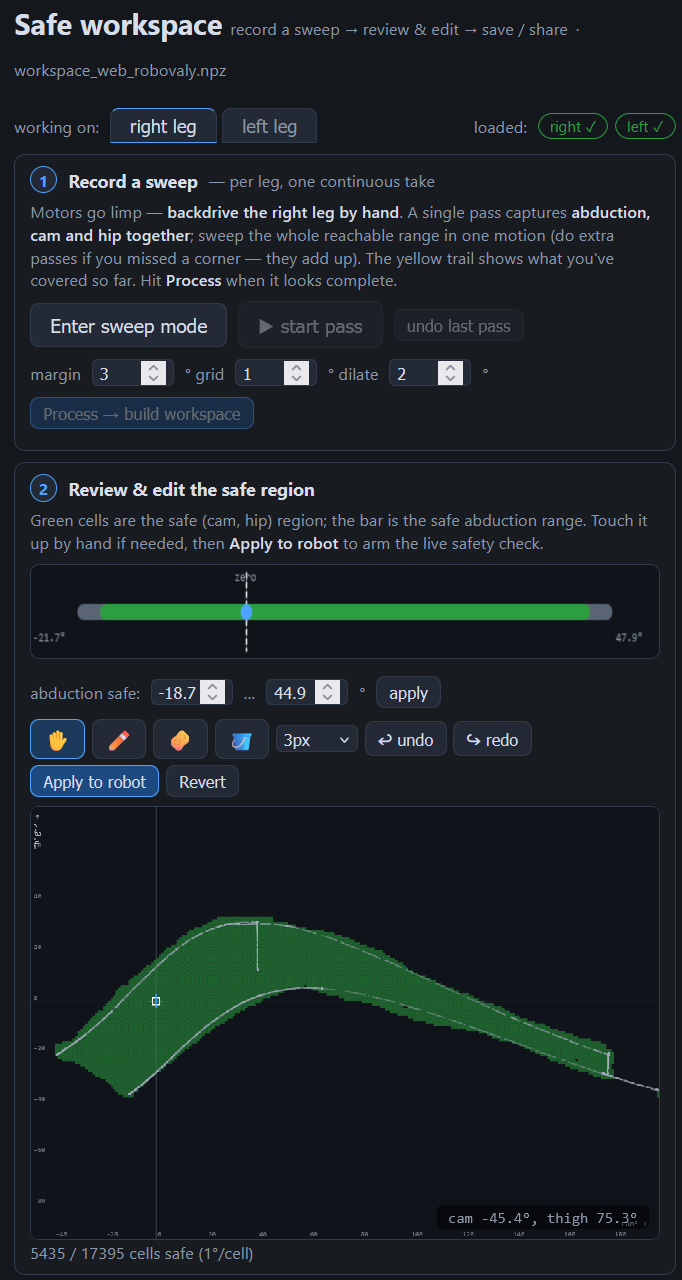
\includegraphics[width=\linewidth]{Figures/fig_WORKSPACEwidget.png}
\captionof{figure}{Workspace widget of the web interface, showing the backdriven joint envelope and the user-drawn safe workspace boundary.}
\label{fig:WORKSPACEwidget}
\end{minipage}\hfill
\begin{minipage}[t]{0.48\linewidth}
\centering
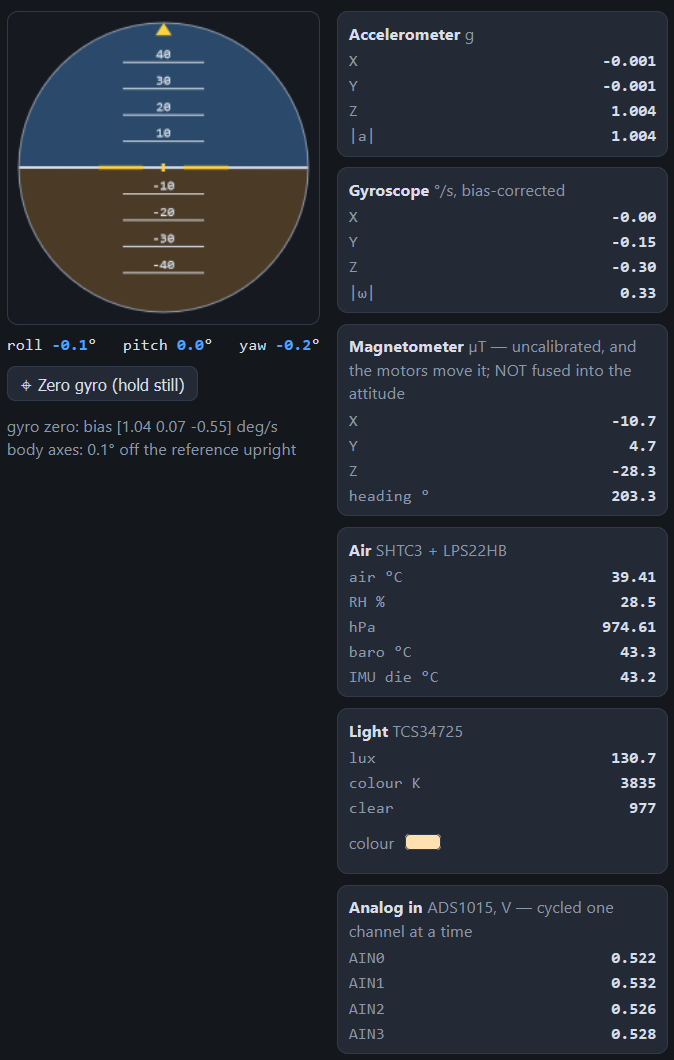
\includegraphics[width=\linewidth]{Figures/fig_IMUwidget.png}
\captionof{figure}{IMU widget of the web interface, used to record accelerometer and gyroscope bias and check axis alignment.}
\label{fig:IMUwidget}
\end{minipage}
\end{figure}


\subsubsection{The safety layer}
\label{sec:safety}

A safety layer was implemented to prevent the robot from exiting the safe operating envelope.
It limits the joint position, the joint speed and the joint torque. If a tracking error greater than a threshold is detected, the robot is stopped.
The user can also at any time stop the robot by clicking the E-STOP button in the web interface.
This safety layer was thoroughly tested in simulation and on the real robot by trying to make the robot exit the safe operating envelope and proved useful on a few occasions to prevent user error.
The safety layer also implements a black-box recorder that records the joint position, speed, torque and the IMU data at 200\,Hz. If a new failure mode is triggered, it will be possible to investigate it.

\subsubsection{Running widget}
\label{sec:hw-experiments}

From the web interface it is possible to both record a gait by backdriving the foot of the robot and then to play it back at a wanted frequency.
This is also where a policy can be selected and run on the robot.


\subsubsection{Measurement widget}
Three widgets carry the plant identification campaign of \cref{sec:plant-id}; \cref{fig:widget-measurement} shows them.
The \emph{thermal identification} widget deposits a known amount of electrical heat in one motor and records the case temperature, to fit a lumped thermal model.
The \emph{dynamic identification} widget excites one leg with workspace-checked position chirps and logs position, velocity and current at 200\,Hz. The recorded runs feed the fit of \cref{sec:inertia-validation}.
The \emph{limbs and inertia} widget stores the weighed segment masses and compares the CAD inertia tensors against the identified ones. The comparison uses the principal moments, which are frame-invariant, so wrong values are told apart from a wrong export frame.

\begin{figure}[H]
\centering
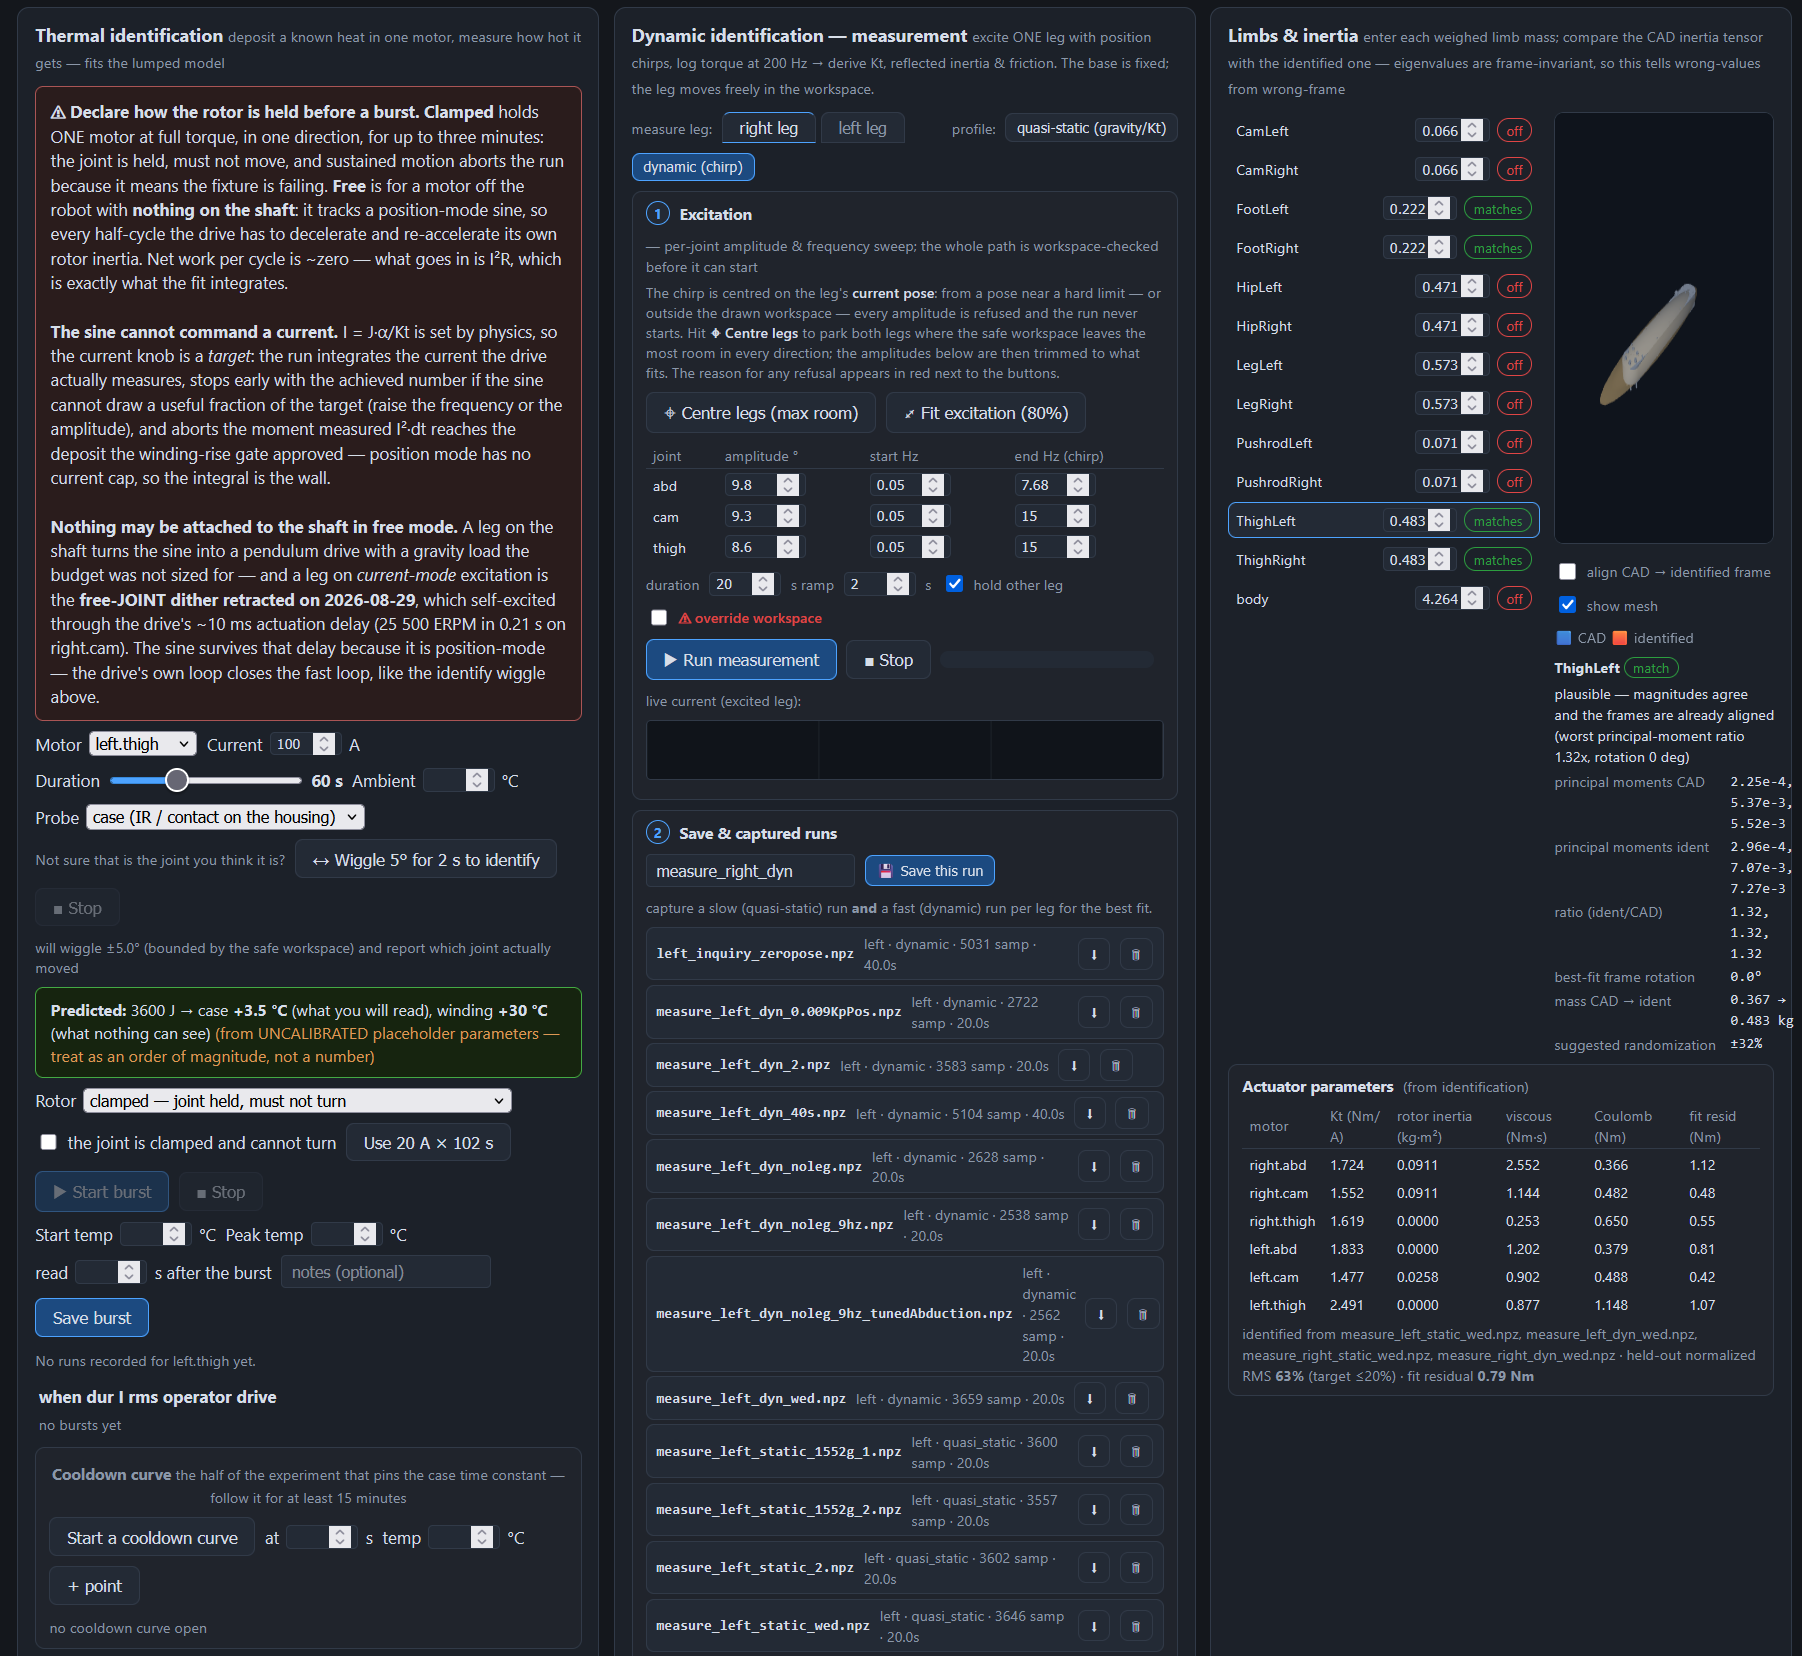
\includegraphics[width=1\linewidth]{Figures/MEASUREMENTSwidget.png}
\caption{The three widgets used to validate the robot parameters and limit the sim2real gap.}
\label{fig:widget-measurement}
\end{figure}


\newpage 

\subsection{Running speed ceiling estimation}
\label{sec:speed-ceiling}

The physical speed ceiling was established independently of reinforcement learning by applying progressively stricter physical constraints to the same robot model.
First,  the body was fixed and ground interaction removed with the leg free to move.
This was used to determine the maximum feasible fore-aft foot sweep over the empirically verified workspace.
The resulting speed was evaluated first from joint-speed limits alone, then with the measured torque-speed envelope and leg inertia, 
and finally with the measured actuator command latency.
This progressively reduced the theoretical ceiling from $14.5\,\mathrm{m/s}$ to $7.4\,\mathrm{m/s}$ and ultimately $6.55\,\mathrm{m/s}$, showing that actuator torque and leg inertia are the dominant limitations.
The result is an optimistic upper bound because the leg carries no body load and balance and contact constraints are ignored.

A second analysis extends the bound to gaits involving a flight phase, where the rail argument no longer applies because ballistic flight can increase stride length.
The maximum speed was instead constrained using an impulse balance: the available vertical foot force, obtained from the leg's force capability, was combined with the minimum time required to execute a stroke.
As speed increases, stance duration decreases while the leg's minimum cycling period remains finite, eventually leaving insufficient stance impulse to support the robot's weight.
This gives a slightly lower upper bound of approximately $6.2\,\mathrm{m/s}$.
Both analyses agree on a ceiling of about 6\,m/s, and this rounded figure is the bound quoted in the rest of the document.
For the details of the simulation, refer to the code itself.\cite{morand2026runningrobot}

\begin{table}[H]
\centering
\small
\begin{tabular}{lrrl}
\toprule
\textbf{Model} & \textbf{Bound} & \textbf{Cost} & \textbf{Binding mechanism} \\
\midrule
Kinematic (no-load speed only)        & 14.5\,m/s  & --      & joint speed through path Jacobian \\
+ torque--speed envelope, inertia     & 7.4\,m/s   & $-49$\,\% & stroke reversals, torque at speed \\
+ 7\,ms MIT-mode latency              & \textbf{6.55\,m/s} & $-12$\,\% & delay caps usable stiffness \\
\midrule
Flight-phase closure (any gait)       & \textbf{6.2\,m/s} & -- & vertical-impulse starvation \\
\bottomrule
\end{tabular}
\caption{The speed ceiling with refined modelling incorporating more realistic physical constraints.}
\label{tab:speed-ceiling}
\end{table}

\begin{figure}[H]
\centering
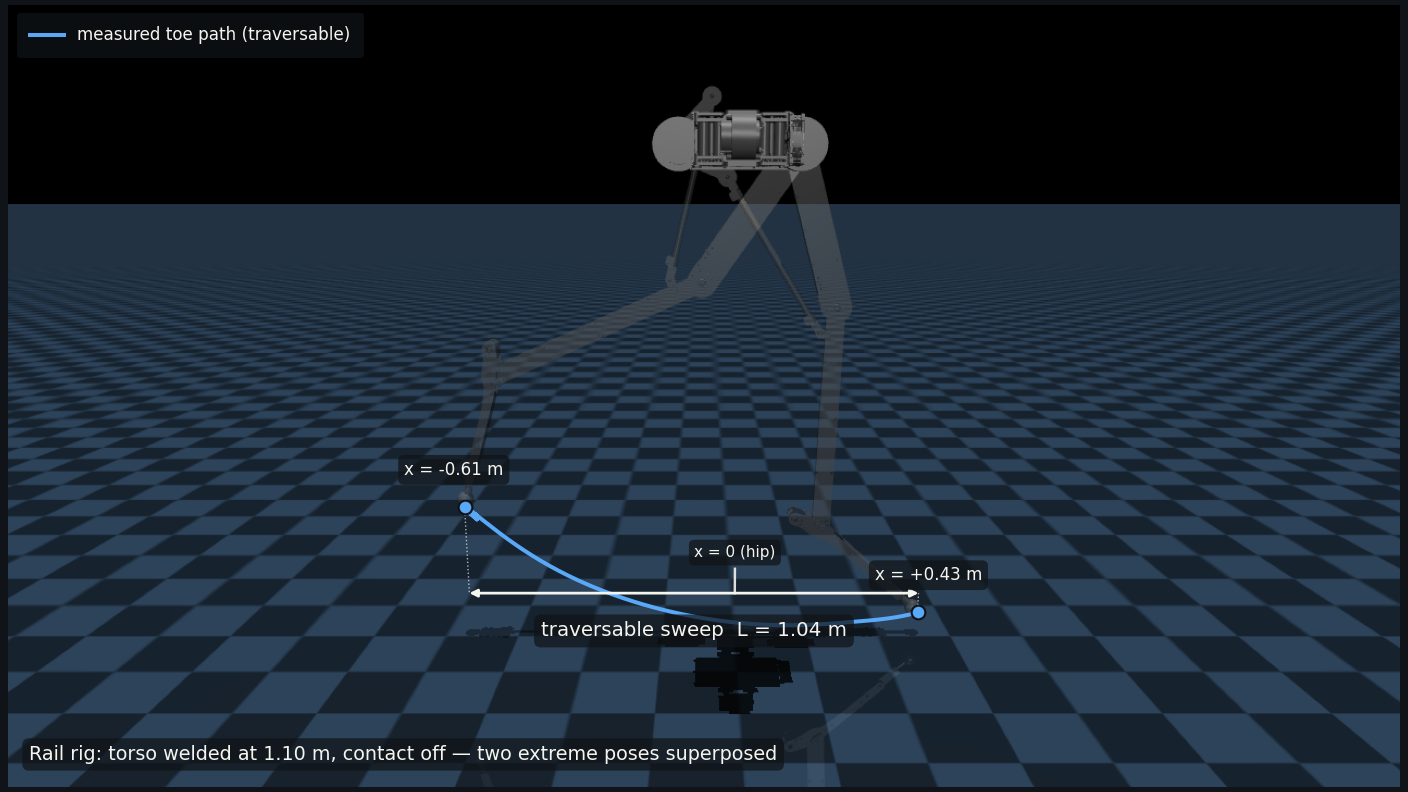
\includegraphics[width=0.85\linewidth]{Figures/rail_sweep_extent.png}
\caption{Workspace of the leg used to infer an optimistic upper bound on the running speed.}
\label{fig:speed-ceiling}
\end{figure}

\subsubsection{Static toe-force map}
\label{sec:plant-id-force}

The speed bound of \cref{sec:speed-ceiling} needs the force the leg can put on the
ground. The leg's static force capability over the measured workspace is therefore mapped.

The domain is the backdriven workspace of \cref{sec:sim-hygiene}. The toe
Jacobian comes from the model's closed-loop forward kinematics (\cref{sec:twin}),
differentiated over a 1\,deg grid. The joint torques are capped at the measured
144.5\,N$\cdot$m of \cref{tab:motors}. The maximum pure-vertical force $F_z$ and
pure-horizontal force $F_x$ at each pose then follow from $\tau = J^\top F$.
Vertical values are clipped at 3.5 body weights as near full extension the leg acts
as a strut, and the Jacobian alone would admit an arbitrary vertical force there.
Poses past the 4-bar's fold boundary are cut, since force there is not usable.

\Cref{fig:force-map} shows the result in body weights (15.14\,kg). The capability
is strongly anisotropic. At the standing pose, near 96\,\% of reach, the force
ellipse is about 19:1: the leg pushes hard straight down and weakly fore-aft,
which is suboptimal for propulsion. The vertical map feeds the impulse
bound of \cref{sec:speed-ceiling}, and the anisotropy makes the linkage
proportions a design lever that is presented in \cref{sec:discussion}.

\begin{figure}[H]
\centering
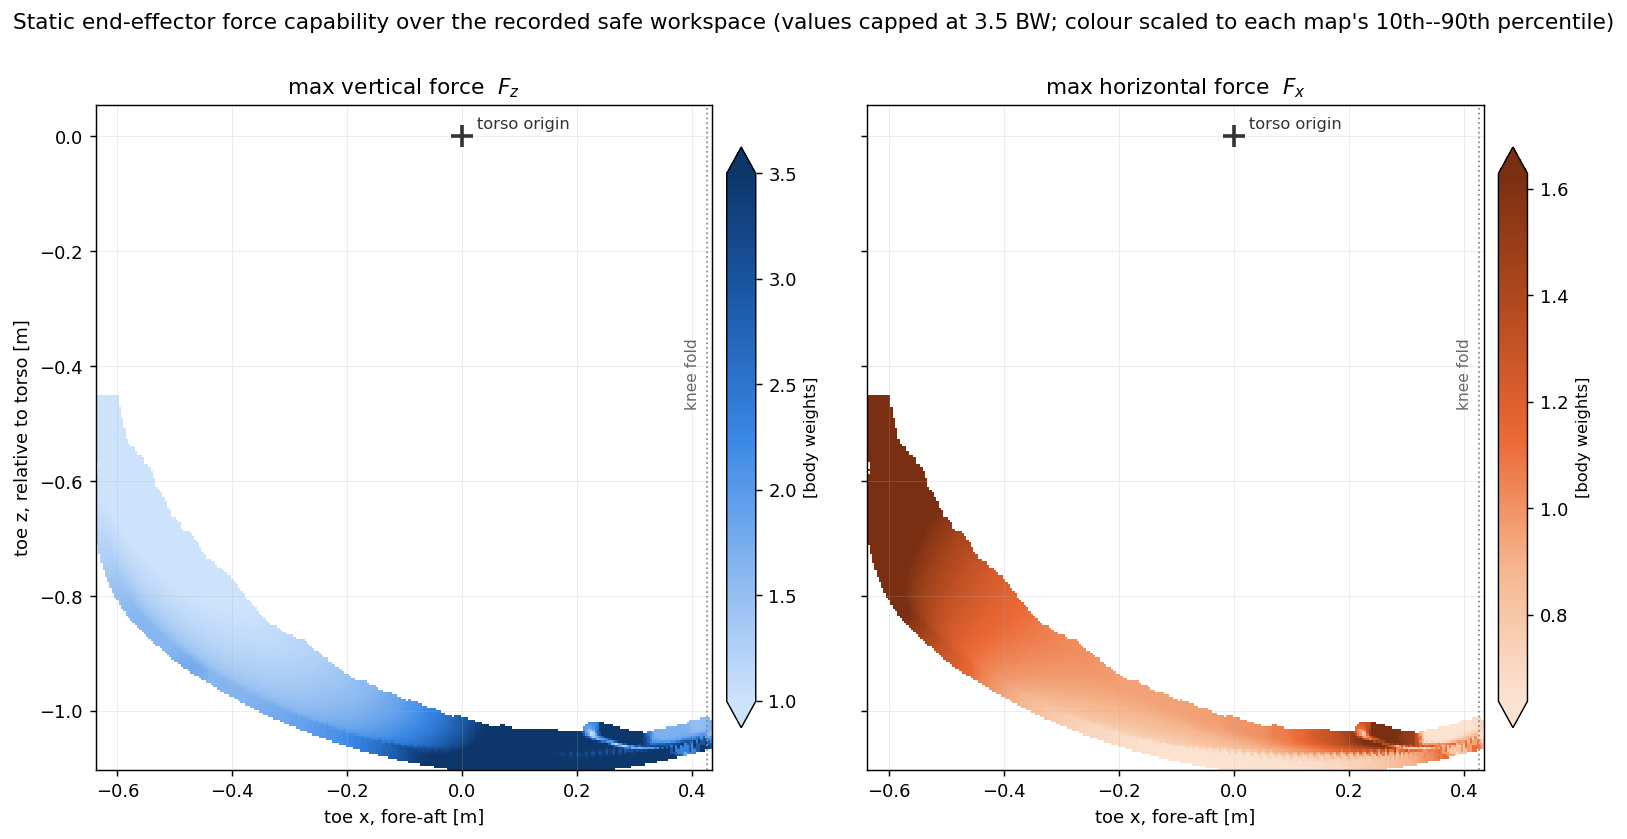
\includegraphics[width=1\linewidth]{Figures/fig_force_map.png}
\caption{Static toe-force capability over the measured workspace: maximum vertical force $F_z$
(left) and horizontal force $F_x$ (right), in body weights, clipped at 3.5\,BW. The vertical map
feeds the flight-phase impulse bound.}
\label{fig:force-map}
\end{figure}


\newpage 

\subsubsection{Sensitivity of the bound to the design parameters}
\label{sec:speed-sensitivity}

The rail model also gives the sensitivity of the bound to the design.
Four parameters were each scaled by $+50\,\%$ with everything else nominal: leg mass, rotor
inertia, deliverable peak torque and bus voltage (through the no-load speed).
Peak torque is the strongest lever: 50\,\% more raises the bound by about 1\,m/s in the worst case and 4\,m/s in the best one.
Leg mass is second: 50\,\% more lowers the bound by about 2\,m/s.
Rotor inertia is nearly flat, and 50\,\% more bus voltage gains nothing, because the bound does not
sit on the no-load-speed ceiling at this operating point.
Leg length was not simulated due to lack of time as it implies updating the URDF, but it is assumed that a longer leg would help increase the stride length.
The levers for a faster robot are therefore deliverable torque and leg mass.
Leg length is also likely a significant lever but its impact and direction are unknown.
\Cref{sec:discussion} ranks the mechanical changes that follow from them, and \cref{sec:rl} trains
its policies against the plant measured in this chapter.


\begin{figure}[H]
  \centering
  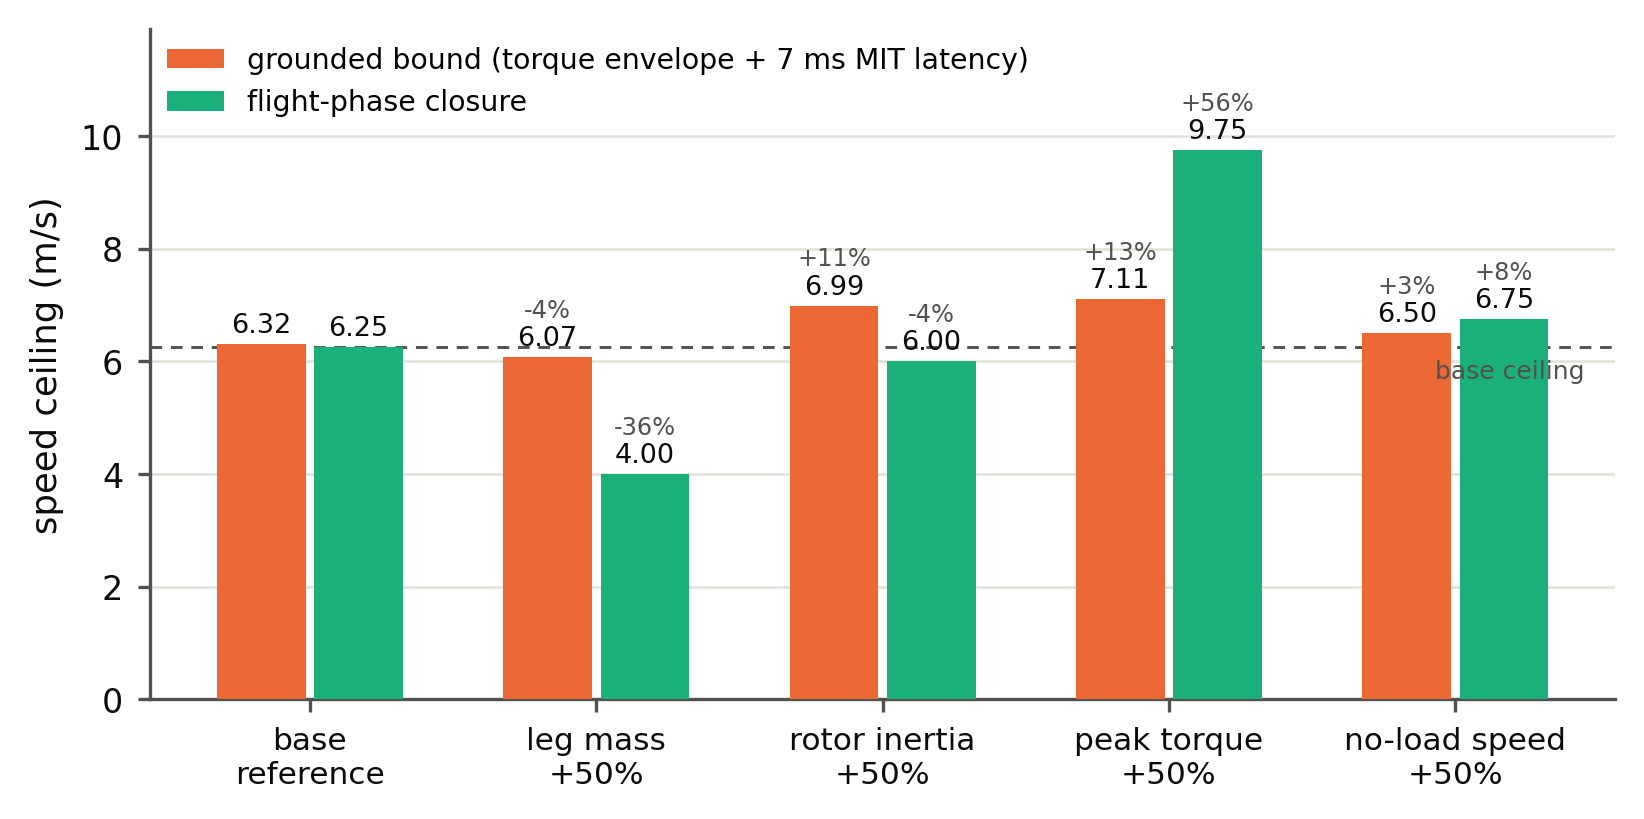
\includegraphics[width=1\textwidth]{Figures/bound_sensitivity_bars.png}
  \caption{Sensitivity of the speed-ceiling estimates to $+50\,\%$ design changes, one
  parameter at a time.}
  \label{fig:bound-sensitivity}
\end{figure}